
為了找到一個對性能的關注從未減弱的例子,讓我們來看看計算的演變(它使計算本身成為可能),\textbf{電子設計自動化(EDA)}工具,其會用來設計計算機。

2010年進行了設計、模擬或驗證某一特定微芯片的計算,此後每年都運行相同的計算量,我們會看到這樣的結果:

%\hspace*{\fill} \\ %插入空行
\begin{center}
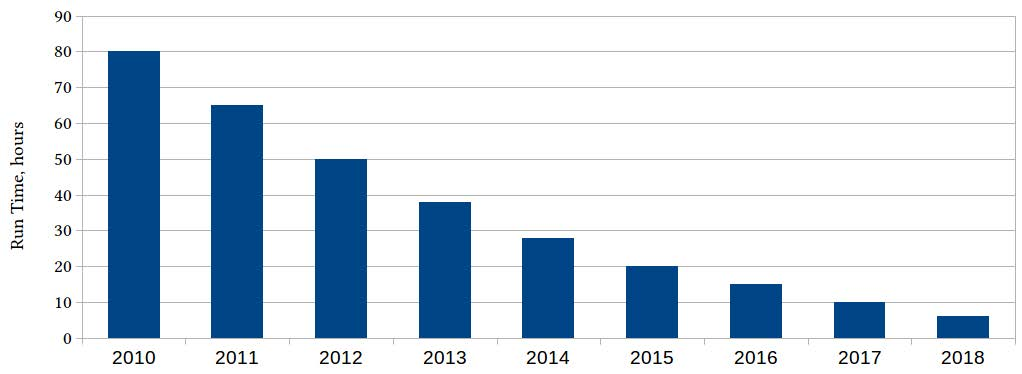
\includegraphics[width=0.9\textwidth]{content/1/chapter1/images/2.jpg}\\
圖1.2 - 這些年來對於特定的EDA計算的處理時間,以小時為單位,
\end{center}

2010年計算時間為80小時,而2018年計算時間不到10小時(現在更短)。改善從何而來?計算機變得更快,但同時軟件變得更高效,使用更好的算法,優化的編譯器變得更高效。

當然,我們不會在2021年製造2010版的微芯片。所以有理由認為,隨著電腦變得越來越強大,製造更新更好的芯片變得越來越困難。那麼,每年要花多長時間才能完成同樣的工作呢?

%\hspace*{\fill} \\ %插入空行
\begin{center}
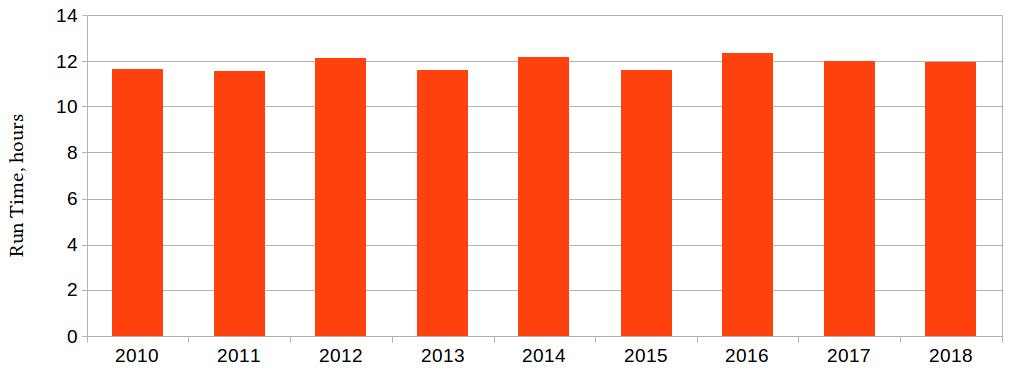
\includegraphics[width=0.9\textwidth]{content/1/chapter1/images/3.jpg}\\
圖1.3 - 每年最新的微芯片的運行時間,以小時為單位
\end{center}

每年實際完成的計算並不相同,但它們的目的相同,例如:對於我們每年製作的芯片,會驗證芯片是否按照預期的方式運行。從這個圖表可以看出,當前最強大的處理器,每年的設計和處理器所用的時間大致相同。雖然我們在努力,但沒有任何進展。

事實比這更糟,上面的圖表並不能說明一切。從2010年到2018年,那一年生產的最大處理器可以在一夜之間(大約12個小時)通過適配去年生產的電腦進行驗證。這裡,我們忘了問有多少個處理器?好吧,下面就是真相:

%\hspace*{\fill} \\ %插入空行
\begin{center}
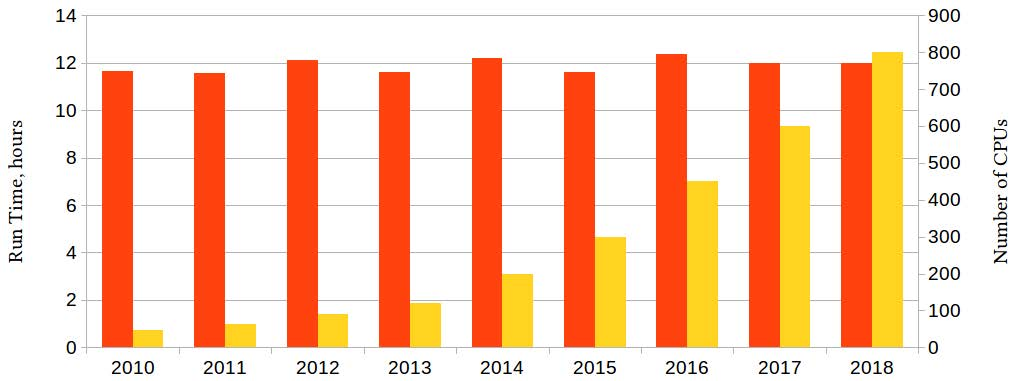
\includegraphics[width=0.9\textwidth]{content/1/chapter1/images/4.jpg}\\
圖1.4 - 添加了每次計算的CPU數量
\end{center}

每年好的計算機,配備了數量不斷增長的處理器,運行最新的軟件(優化會利用越來越多的處理器,並更有效地使用每個處理器),完成構造下一年計算機所需的工作。每年都是在這樣,但這項任務幾乎不可能完成。我們依靠硬件和軟件工程師的成就保持一優勢,因為前者提供了不斷增長的計算能力,而後者則以最高的效率使用它。這本書將來瞭解後者所使用的相關技能。

我們現在瞭解了這本書中內容的重要性。在深入研究細節之前,做一個概述可能會有所幫助。


















